\documentclass[]{article}
\usepackage{lmodern}
\usepackage{amssymb,amsmath}
\usepackage{ifxetex,ifluatex}
\usepackage{fixltx2e} % provides \textsubscript
\ifnum 0\ifxetex 1\fi\ifluatex 1\fi=0 % if pdftex
  \usepackage[T1]{fontenc}
  \usepackage[utf8]{inputenc}
\else % if luatex or xelatex
  \ifxetex
    \usepackage{mathspec}
  \else
    \usepackage{fontspec}
  \fi
  \defaultfontfeatures{Ligatures=TeX,Scale=MatchLowercase}
\fi
% use upquote if available, for straight quotes in verbatim environments
\IfFileExists{upquote.sty}{\usepackage{upquote}}{}
% use microtype if available
\IfFileExists{microtype.sty}{%
\usepackage{microtype}
\UseMicrotypeSet[protrusion]{basicmath} % disable protrusion for tt fonts
}{}
\usepackage[margin=1.5cm]{geometry}
\usepackage{hyperref}
\hypersetup{unicode=true,
            pdftitle={Atlas-PS 2},
            pdfauthor={David Atlas},
            pdfborder={0 0 0},
            breaklinks=true}
\urlstyle{same}  % don't use monospace font for urls
\usepackage{color}
\usepackage{fancyvrb}
\newcommand{\VerbBar}{|}
\newcommand{\VERB}{\Verb[commandchars=\\\{\}]}
\DefineVerbatimEnvironment{Highlighting}{Verbatim}{commandchars=\\\{\}}
% Add ',fontsize=\small' for more characters per line
\usepackage{framed}
\definecolor{shadecolor}{RGB}{248,248,248}
\newenvironment{Shaded}{\begin{snugshade}}{\end{snugshade}}
\newcommand{\KeywordTok}[1]{\textcolor[rgb]{0.13,0.29,0.53}{\textbf{#1}}}
\newcommand{\DataTypeTok}[1]{\textcolor[rgb]{0.13,0.29,0.53}{#1}}
\newcommand{\DecValTok}[1]{\textcolor[rgb]{0.00,0.00,0.81}{#1}}
\newcommand{\BaseNTok}[1]{\textcolor[rgb]{0.00,0.00,0.81}{#1}}
\newcommand{\FloatTok}[1]{\textcolor[rgb]{0.00,0.00,0.81}{#1}}
\newcommand{\ConstantTok}[1]{\textcolor[rgb]{0.00,0.00,0.00}{#1}}
\newcommand{\CharTok}[1]{\textcolor[rgb]{0.31,0.60,0.02}{#1}}
\newcommand{\SpecialCharTok}[1]{\textcolor[rgb]{0.00,0.00,0.00}{#1}}
\newcommand{\StringTok}[1]{\textcolor[rgb]{0.31,0.60,0.02}{#1}}
\newcommand{\VerbatimStringTok}[1]{\textcolor[rgb]{0.31,0.60,0.02}{#1}}
\newcommand{\SpecialStringTok}[1]{\textcolor[rgb]{0.31,0.60,0.02}{#1}}
\newcommand{\ImportTok}[1]{#1}
\newcommand{\CommentTok}[1]{\textcolor[rgb]{0.56,0.35,0.01}{\textit{#1}}}
\newcommand{\DocumentationTok}[1]{\textcolor[rgb]{0.56,0.35,0.01}{\textbf{\textit{#1}}}}
\newcommand{\AnnotationTok}[1]{\textcolor[rgb]{0.56,0.35,0.01}{\textbf{\textit{#1}}}}
\newcommand{\CommentVarTok}[1]{\textcolor[rgb]{0.56,0.35,0.01}{\textbf{\textit{#1}}}}
\newcommand{\OtherTok}[1]{\textcolor[rgb]{0.56,0.35,0.01}{#1}}
\newcommand{\FunctionTok}[1]{\textcolor[rgb]{0.00,0.00,0.00}{#1}}
\newcommand{\VariableTok}[1]{\textcolor[rgb]{0.00,0.00,0.00}{#1}}
\newcommand{\ControlFlowTok}[1]{\textcolor[rgb]{0.13,0.29,0.53}{\textbf{#1}}}
\newcommand{\OperatorTok}[1]{\textcolor[rgb]{0.81,0.36,0.00}{\textbf{#1}}}
\newcommand{\BuiltInTok}[1]{#1}
\newcommand{\ExtensionTok}[1]{#1}
\newcommand{\PreprocessorTok}[1]{\textcolor[rgb]{0.56,0.35,0.01}{\textit{#1}}}
\newcommand{\AttributeTok}[1]{\textcolor[rgb]{0.77,0.63,0.00}{#1}}
\newcommand{\RegionMarkerTok}[1]{#1}
\newcommand{\InformationTok}[1]{\textcolor[rgb]{0.56,0.35,0.01}{\textbf{\textit{#1}}}}
\newcommand{\WarningTok}[1]{\textcolor[rgb]{0.56,0.35,0.01}{\textbf{\textit{#1}}}}
\newcommand{\AlertTok}[1]{\textcolor[rgb]{0.94,0.16,0.16}{#1}}
\newcommand{\ErrorTok}[1]{\textcolor[rgb]{0.64,0.00,0.00}{\textbf{#1}}}
\newcommand{\NormalTok}[1]{#1}
\usepackage{longtable,booktabs}
\usepackage{graphicx,grffile}
\makeatletter
\def\maxwidth{\ifdim\Gin@nat@width>\linewidth\linewidth\else\Gin@nat@width\fi}
\def\maxheight{\ifdim\Gin@nat@height>\textheight\textheight\else\Gin@nat@height\fi}
\makeatother
% Scale images if necessary, so that they will not overflow the page
% margins by default, and it is still possible to overwrite the defaults
% using explicit options in \includegraphics[width, height, ...]{}
\setkeys{Gin}{width=\maxwidth,height=\maxheight,keepaspectratio}
\IfFileExists{parskip.sty}{%
\usepackage{parskip}
}{% else
\setlength{\parindent}{0pt}
\setlength{\parskip}{6pt plus 2pt minus 1pt}
}
\setlength{\emergencystretch}{3em}  % prevent overfull lines
\providecommand{\tightlist}{%
  \setlength{\itemsep}{0pt}\setlength{\parskip}{0pt}}
\setcounter{secnumdepth}{0}
% Redefines (sub)paragraphs to behave more like sections
\ifx\paragraph\undefined\else
\let\oldparagraph\paragraph
\renewcommand{\paragraph}[1]{\oldparagraph{#1}\mbox{}}
\fi
\ifx\subparagraph\undefined\else
\let\oldsubparagraph\subparagraph
\renewcommand{\subparagraph}[1]{\oldsubparagraph{#1}\mbox{}}
\fi

%%% Use protect on footnotes to avoid problems with footnotes in titles
\let\rmarkdownfootnote\footnote%
\def\footnote{\protect\rmarkdownfootnote}

%%% Change title format to be more compact
\usepackage{titling}

% Create subtitle command for use in maketitle
\newcommand{\subtitle}[1]{
  \posttitle{
    \begin{center}\large#1\end{center}
    }
}

\setlength{\droptitle}{-2em}

  \title{Atlas-PS 2}
    \pretitle{\vspace{\droptitle}\centering\huge}
  \posttitle{\par}
    \author{David Atlas}
    \preauthor{\centering\large\emph}
  \postauthor{\par}
    \date{}
    \predate{}\postdate{}
  

\begin{document}
\maketitle

\newcommand{\summ}{\Sigma_{i=1}^{n}}

\section{Problem 1}\label{problem-1}

\subsection{a)}\label{a}

Let \(X = (28, 33, 22, 35)\) be our set of i.i.d data points. The
function \(s_p(\theta)=\sqrt{\Sigma_{x \in X}(\theta - x)^2}\), or the
sum of squared residuals.

\subsection{b)}\label{b}

\(s_p(\theta)\) is plotted below, with the R code used to generate the
plot.

\begin{Shaded}
\begin{Highlighting}[]
\NormalTok{x <-}\StringTok{ }\KeywordTok{c}\NormalTok{(}\DecValTok{28}\NormalTok{, }\DecValTok{33}\NormalTok{, }\DecValTok{22}\NormalTok{, }\DecValTok{35}\NormalTok{)}
\NormalTok{s_p <-}\StringTok{ }\ControlFlowTok{function}\NormalTok{(theta, x)\{}
  \CommentTok{# We implement our function to minimize}
  \KeywordTok{return}\NormalTok{(}\KeywordTok{sqrt}\NormalTok{(}\KeywordTok{sum}\NormalTok{((theta }\OperatorTok{-}\StringTok{ }\NormalTok{x) }\OperatorTok{^}\StringTok{ }\DecValTok{2}\NormalTok{)))}
\NormalTok{\}}

\CommentTok{# We set up our domain for theta}
\NormalTok{theta_space <-}\StringTok{ }\KeywordTok{seq}\NormalTok{(}\DecValTok{20}\NormalTok{, }\DecValTok{35}\NormalTok{, .}\DecValTok{25}\NormalTok{)}
\CommentTok{# We calculate the function value over the space}
\NormalTok{s_p_theta_space <-}\StringTok{ }\KeywordTok{sapply}\NormalTok{(theta_space, }\ControlFlowTok{function}\NormalTok{(theta)\{}\KeywordTok{s_p}\NormalTok{(theta, x)\})}

\CommentTok{# We plot the function over the space}
\KeywordTok{plot}\NormalTok{(theta_space, s_p_theta_space, }\StringTok{'l'}\NormalTok{, }
  \DataTypeTok{main=}\KeywordTok{TeX}\NormalTok{(}\StringTok{'Plot of $s_p(}\CharTok{\textbackslash{}\textbackslash{}}\StringTok{Theta)$'}\NormalTok{), }
  \DataTypeTok{xlab=}\KeywordTok{TeX}\NormalTok{(}\StringTok{'$}\CharTok{\textbackslash{}\textbackslash{}}\StringTok{theta$'}\NormalTok{), }\DataTypeTok{ylab=}\KeywordTok{TeX}\NormalTok{(}\StringTok{'$s_p(}\CharTok{\textbackslash{}\textbackslash{}}\StringTok{theta)$'}\NormalTok{))}
\end{Highlighting}
\end{Shaded}

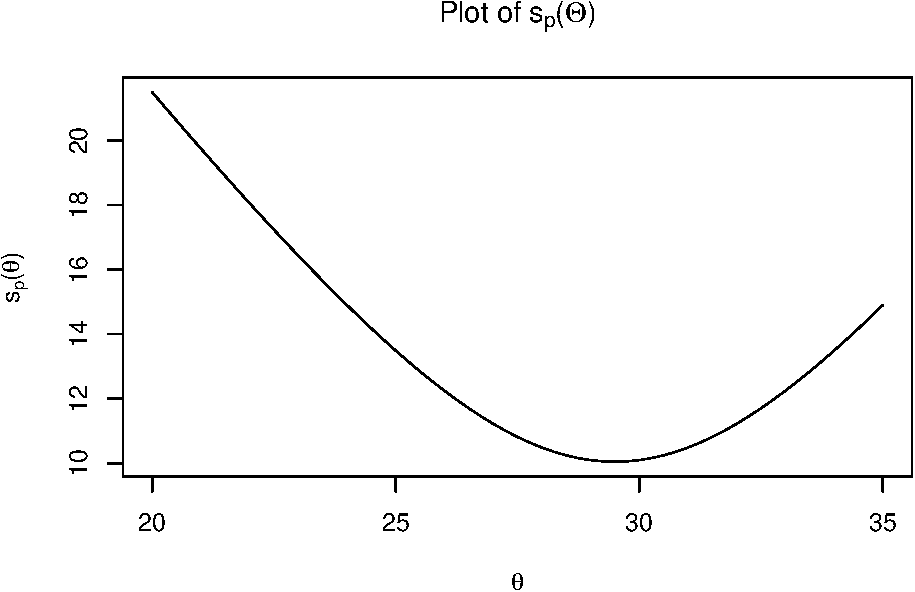
\includegraphics{Atlas-PS_2_files/figure-latex/unnamed-chunk-1-1.pdf}

\subsection{c)}\label{c}

To use the bisection method, we must first compute
\(s_p\prime(\theta)\).

\begin{align*}
  s_p\prime (\theta) &= \frac{1}{2} (\Sigma_{x \in X} (\theta - x)^{2})^{-\frac{1}{2}} \times 2 \Sigma_{x\in X}(\theta-x) \\
  &= (\Sigma_{x \in X} (\theta - x)^{2})^{-\frac{1}{2}} \Sigma_{x\in X}(\theta - x).
\end{align*}

Next, we implement the bisection method, as well as \(s_p(\theta)\) and
\(s_p \prime (\theta)\). We plot the \(s_p(\theta)\) with the Minimum
Residual Estimator as a vertical line. The solution to the optimization
problem is \(\hat{\theta}=29.50\).

\begin{Shaded}
\begin{Highlighting}[]
\NormalTok{x <-}\StringTok{ }\KeywordTok{c}\NormalTok{(}\DecValTok{28}\NormalTok{, }\DecValTok{33}\NormalTok{, }\DecValTok{22}\NormalTok{, }\DecValTok{35}\NormalTok{)}

\NormalTok{s_p <-}\StringTok{ }\ControlFlowTok{function}\NormalTok{(theta, x)\{}
  \CommentTok{# We implement our function to minimize}
  \KeywordTok{return}\NormalTok{(}\KeywordTok{sqrt}\NormalTok{(}\KeywordTok{sum}\NormalTok{((theta }\OperatorTok{-}\StringTok{ }\NormalTok{x) }\OperatorTok{^}\StringTok{ }\DecValTok{2}\NormalTok{)))}
\NormalTok{\}}

\NormalTok{s_p_prime <-}\StringTok{ }\ControlFlowTok{function}\NormalTok{(theta, x)\{}
  \CommentTok{# This is the first derivative of the function}
  \KeywordTok{return}\NormalTok{(((}\KeywordTok{sum}\NormalTok{(theta }\OperatorTok{-}\StringTok{ }\NormalTok{x) }\OperatorTok{^}\StringTok{ }\DecValTok{2}\NormalTok{) }\OperatorTok{^}\StringTok{ }\OperatorTok{-}\NormalTok{.}\DecValTok{5}\NormalTok{) }\OperatorTok{*}\StringTok{ }\KeywordTok{sum}\NormalTok{(theta }\OperatorTok{-}\StringTok{ }\NormalTok{x))}
\NormalTok{\}}

\NormalTok{bisection <-}\StringTok{ }\ControlFlowTok{function}\NormalTok{(a, b, f_prime, }\DataTypeTok{tol=}\NormalTok{.}\DecValTok{0001}\NormalTok{, }\DataTypeTok{n=}\DecValTok{0}\NormalTok{)\{}
\NormalTok{  x_t <-}\StringTok{ }\NormalTok{.}\DecValTok{5} \OperatorTok{*}\StringTok{ }\NormalTok{(a }\OperatorTok{+}\StringTok{ }\NormalTok{b)}
  \CommentTok{# Use conditioning to get the next interval}
  \ControlFlowTok{if}\NormalTok{(}\KeywordTok{f_prime}\NormalTok{(a, x) }\OperatorTok{*}\StringTok{ }\KeywordTok{f_prime}\NormalTok{(x_t, x) }\OperatorTok{<=}\StringTok{ }\DecValTok{0}\NormalTok{)\{}
\NormalTok{    new_interval <-}\StringTok{ }\KeywordTok{c}\NormalTok{(a, x_t)}
\NormalTok{  \}}\ControlFlowTok{else}\NormalTok{\{}
\NormalTok{    new_interval <-}\StringTok{ }\KeywordTok{c}\NormalTok{(x_t, b)}
\NormalTok{  \}}
  
  \CommentTok{# if interval is less than the tolerance, stop the recursion.}
  \ControlFlowTok{if}\NormalTok{ ((b }\OperatorTok{-}\StringTok{ }\NormalTok{a) }\OperatorTok{<}\StringTok{ }\NormalTok{tol)\{}
    \KeywordTok{print}\NormalTok{(}\KeywordTok{paste0}\NormalTok{(}\StringTok{"The solution is "}\NormalTok{, }\KeywordTok{round}\NormalTok{(x_t, }\DecValTok{3}\NormalTok{) , }\StringTok{" and it was found in "}\NormalTok{, n, }\StringTok{" iterations."}\NormalTok{))}
    \KeywordTok{return}\NormalTok{(x_t)}
\NormalTok{  \}}\ControlFlowTok{else}\NormalTok{\{}
    \CommentTok{# If not, call again on the new interval}
    \KeywordTok{return}\NormalTok{(}\KeywordTok{bisection}\NormalTok{(new_interval[}\DecValTok{1}\NormalTok{], new_interval[}\DecValTok{2}\NormalTok{], f_prime, }\DataTypeTok{n=}\NormalTok{n }\OperatorTok{+}\StringTok{ }\DecValTok{1}\NormalTok{))  }
\NormalTok{  \}}
\NormalTok{\}}

\KeywordTok{plot}\NormalTok{(theta_space, s_p_theta_space, }\StringTok{'l'}\NormalTok{, }
  \DataTypeTok{main=}\KeywordTok{TeX}\NormalTok{(}\StringTok{'Plot of $s_p(}\CharTok{\textbackslash{}\textbackslash{}}\StringTok{Theta)$'}\NormalTok{), }
  \DataTypeTok{xlab=}\KeywordTok{TeX}\NormalTok{(}\StringTok{'$}\CharTok{\textbackslash{}\textbackslash{}}\StringTok{theta$'}\NormalTok{), }\DataTypeTok{ylab=}\KeywordTok{TeX}\NormalTok{(}\StringTok{'$s_p(}\CharTok{\textbackslash{}\textbackslash{}}\StringTok{theta)$'}\NormalTok{))}
\KeywordTok{abline}\NormalTok{(}\DataTypeTok{v=}\KeywordTok{bisection}\NormalTok{(}\DecValTok{20}\NormalTok{, }\DecValTok{35}\NormalTok{, s_p_prime, }\DataTypeTok{tol=}\NormalTok{.}\DecValTok{000001}\NormalTok{))}
\end{Highlighting}
\end{Shaded}

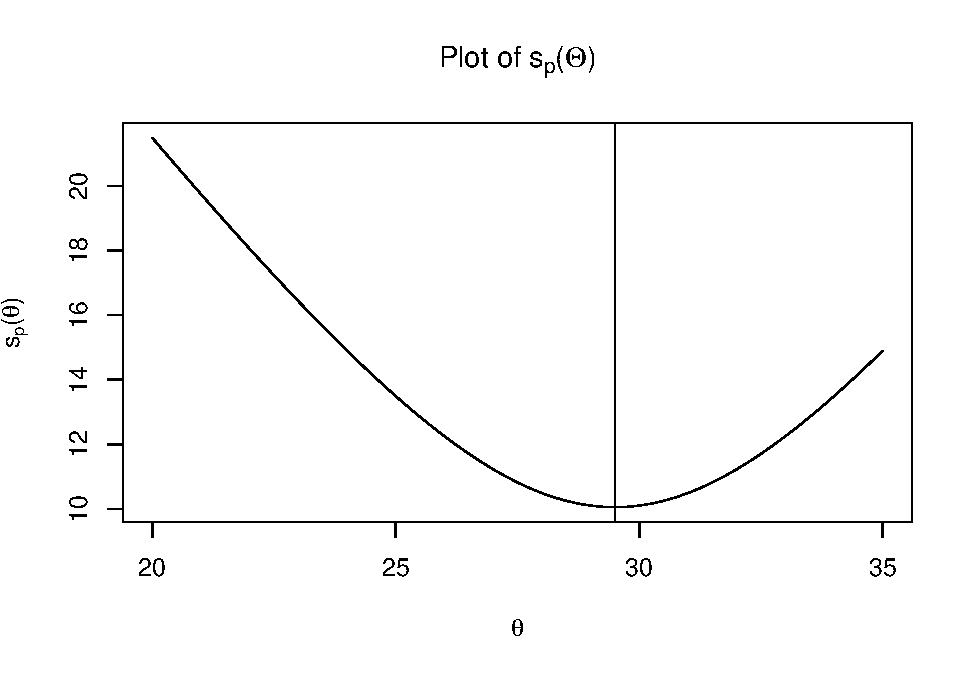
\includegraphics{Atlas-PS_2_files/figure-latex/unnamed-chunk-2-1.pdf}

\begin{verbatim}
## [1] "The solution is 29.5 and it was found in 18 iterations."
\end{verbatim}

\subsection{d)}\label{d}

We already calculated
\(s_p^\prime (\theta) = (\Sigma_{x \in X} (\theta - x)^{2})^{-\frac{1}{2}}\Sigma_{x\in X}(\theta - x)\).
We find

\begin{align*}
s_p^{\prime \prime} (\theta) &= -\frac{1}{2} (\Sigma_{x \in X} (\theta - x)^2)^{-\frac{3}{2}}
\Sigma_{x \in X}(\theta - x) +  (\Sigma_{x \in X} (\theta - x)^2)^{-\frac{1}{2}}.
\end{align*}

We can then find
\(h(\theta) = \frac{s_p^{\prime}(\theta)}{s_p^{\prime \prime}(\theta)}\).

\begin{align*}
  -\frac{s_p^{\prime}(\theta)}{s_p^{\prime \prime}(\theta)} &=
    -\frac{(\Sigma_{x \in X} (\theta - x)^{2})^{-\frac{1}{2}}\Sigma_{x\in X}(\theta - x)}
      {-\frac{1}{2} (\Sigma_{x \in X} (\theta - x)^2)^{-\frac{3}{2}}
      \Sigma_{x \in X}(\theta - x) +  (\Sigma_{x \in X} (\theta - x)^2)^{-\frac{1}{2}}} \\
      &= 2 \frac{\Sigma_{x \in X}(\theta - x)}{\Sigma_{x \in X}(\theta - x)^2 + 2}
\end{align*}

\section{Problem 2}\label{problem-2}

We maximize the function
\(f(x) = -\frac{x^4}{4} + \frac{x^2}{2} - x + 2\) using Newton's Method
and starting points \(x_0=-1\) and \(x_0=2\). We also print out the
number of iterations needed to converge within 2 decimal places. We
define the first 2 derivatives of the function below:

\begin{align}
f(x) &= -\frac{x^4}{4} + \frac{x^2}{2} - x + 2 \\ 
f^{\prime}(x) &= -x^3+ x - 1 \\ 
f^{\prime \prime}(x) &= -3x^2 + 1
\end{align}

We implement Newton's Method:

\begin{Shaded}
\begin{Highlighting}[]
\NormalTok{newtons <-}\StringTok{ }\ControlFlowTok{function}\NormalTok{(xt, fprime, f2prime, }\DataTypeTok{n=}\DecValTok{1}\NormalTok{, }\DataTypeTok{tol=}\FloatTok{0.01}\NormalTok{)\{}
  \CommentTok{# Define the updating equation}
\NormalTok{  xt_update <-}\StringTok{ }\NormalTok{xt }\OperatorTok{-}\StringTok{ }\NormalTok{(}\KeywordTok{fprime}\NormalTok{(xt) }\OperatorTok{/}\StringTok{ }\KeywordTok{f2prime}\NormalTok{(xt))}
  
  \CommentTok{# If the adjustment value is less than the tolerance, end the iterations}
  \ControlFlowTok{if}\NormalTok{(}\KeywordTok{abs}\NormalTok{(xt_update }\OperatorTok{-}\StringTok{ }\NormalTok{xt) }\OperatorTok{<}\StringTok{ }\NormalTok{tol)\{}
    \KeywordTok{print}\NormalTok{(}\KeywordTok{paste0}\NormalTok{(}\StringTok{"The solution is "}\NormalTok{, }\KeywordTok{round}\NormalTok{(xt_update, }\DecValTok{3}\NormalTok{) , }\StringTok{" and it was found in "}\NormalTok{, n, }\StringTok{" iterations."}\NormalTok{))}
    \KeywordTok{return}\NormalTok{(xt_update)}
\NormalTok{  \}}\ControlFlowTok{else}\NormalTok{\{}
    \CommentTok{# If not, call the recursive formula again}
    \KeywordTok{return}\NormalTok{(}\KeywordTok{newtons}\NormalTok{(xt_update, fprime, f2prime, }\DataTypeTok{n=}\NormalTok{n}\OperatorTok{+}\DecValTok{1}\NormalTok{, }\DataTypeTok{tol=}\NormalTok{tol))}
\NormalTok{  \}}
\NormalTok{\}}

\NormalTok{fprime <-}\StringTok{ }\ControlFlowTok{function}\NormalTok{(x)\{}
  \KeywordTok{return}\NormalTok{(}\OperatorTok{-}\NormalTok{x}\OperatorTok{^}\DecValTok{3} \OperatorTok{+}\StringTok{ }\NormalTok{x }\OperatorTok{-}\DecValTok{1}\NormalTok{)}
\NormalTok{\}}

\NormalTok{f2prime <-}\StringTok{ }\ControlFlowTok{function}\NormalTok{(x)\{}
  \KeywordTok{return}\NormalTok{(}\OperatorTok{-}\DecValTok{3} \OperatorTok{*}\StringTok{ }\NormalTok{x }\OperatorTok{^}\StringTok{ }\DecValTok{2} \OperatorTok{+}\StringTok{ }\DecValTok{1}\NormalTok{)}
\NormalTok{\}}
\end{Highlighting}
\end{Shaded}

\subsection{a)}\label{a-1}

We solve the optimization using \(x_0=-1\).

\begin{Shaded}
\begin{Highlighting}[]
\NormalTok{x0 <-}\StringTok{ }\OperatorTok{-}\DecValTok{1}
\NormalTok{solution <-}\StringTok{ }\KeywordTok{newtons}\NormalTok{(x0, fprime, f2prime)}
\end{Highlighting}
\end{Shaded}

\begin{verbatim}
## [1] "The solution is -1.325 and it was found in 4 iterations."
\end{verbatim}

The solution is -1.325, and it took 4 iterations to find it.

\subsection{b)}\label{b-1}

We solve the optimization using \(x_0=2\).

\begin{Shaded}
\begin{Highlighting}[]
\NormalTok{x0 <-}\StringTok{ }\DecValTok{2}
\NormalTok{solution <-}\StringTok{ }\KeywordTok{newtons}\NormalTok{(x0, fprime, f2prime)}
\end{Highlighting}
\end{Shaded}

\begin{verbatim}
## [1] "The solution is -1.325 and it was found in 64 iterations."
\end{verbatim}

The solution is -1.325, and it took 64 iterations to find it.

\section{Problem 3}\label{problem-3}

We solve exercise 2.1 from the textbook:

The following data are an i.i.d. sample from a Cauchy(\(\theta\), 1)
distribution: 1.77, -.23, 2.76, 3.80, 3.47, 56.75, -1.34, 4.24, -2.44,
3.29, 3.71, -2.40, 4.53, -.07, -1.05, -13.87, -2.53, -1.75, .27, 43.21.

\subsection{a)}\label{a-2}

Graph the log likelihood function. Find the MLE for \(\theta\) using the
Newton-Raphson method. Try the following starting point: -11, -1, 0,
1.5, 4, 4.7, 7, 8, 38. Discuss your results. Is the mean of the data a
good starting point?

The likelihood function of a Cauchy(\(\theta\), 1) distribution: \[
L(\theta) = \prod_{x \in X} \frac{1}
{\pi(1 + (x - \theta) ^ 2)}.
\] Therefore, the log-likelihood is

\begin{align*}
l(\theta) &= \Sigma_{x \in X}\ln\left(\frac{1}{\pi (1 + (x - \theta)^2)}\right) \\&= \Sigma_{x \in X} -\ln(\pi(1  + (x - \theta)^2)) \\
&= - n \ln(\pi) - \Sigma_{x \in X} \ln(1 + (x - \theta) ^ 2),
\end{align*}

where \(n\) is the number of observations in \(X\).

We plot the function below.

\begin{Shaded}
\begin{Highlighting}[]
\NormalTok{X <-}\StringTok{ }\KeywordTok{c}\NormalTok{(}\FloatTok{1.77}\NormalTok{, }\OperatorTok{-}\NormalTok{.}\DecValTok{23}\NormalTok{, }\FloatTok{2.76}\NormalTok{, }\FloatTok{3.80}\NormalTok{, }\FloatTok{3.47}\NormalTok{, }\FloatTok{56.75}\NormalTok{, }\OperatorTok{-}\FloatTok{1.34}\NormalTok{, }\FloatTok{4.24}\NormalTok{, }
\OperatorTok{-}\FloatTok{2.44}\NormalTok{, }\FloatTok{3.29}\NormalTok{, }\FloatTok{3.71}\NormalTok{, }\OperatorTok{-}\FloatTok{2.40}\NormalTok{, }\FloatTok{4.53}\NormalTok{, }\OperatorTok{-}\NormalTok{.}\DecValTok{07}\NormalTok{, }\OperatorTok{-}\FloatTok{1.05}\NormalTok{, }\OperatorTok{-}\FloatTok{13.87}\NormalTok{, }
\OperatorTok{-}\FloatTok{2.53}\NormalTok{, }\OperatorTok{-}\FloatTok{1.75}\NormalTok{, .}\DecValTok{27}\NormalTok{, }\FloatTok{43.21}\NormalTok{)}

\NormalTok{log_likelihood <-}\StringTok{ }\ControlFlowTok{function}\NormalTok{(theta, x)\{}
  \KeywordTok{return}\NormalTok{ (}\KeywordTok{sum}\NormalTok{(}\KeywordTok{dcauchy}\NormalTok{(x, }\DataTypeTok{location=}\NormalTok{theta, }\DataTypeTok{scale=}\DecValTok{1}\NormalTok{, }\DataTypeTok{log=}\OtherTok{TRUE}\NormalTok{)))}
\NormalTok{\}}

\CommentTok{# Create a space for theta}
\NormalTok{theta_space <-}\StringTok{ }\KeywordTok{seq}\NormalTok{(}\OperatorTok{-}\DecValTok{50}\NormalTok{, }\DecValTok{100}\NormalTok{, .}\DecValTok{25}\NormalTok{)}

\CommentTok{# Create the function results for theta}
\NormalTok{theta_f <-}\StringTok{ }\KeywordTok{sapply}\NormalTok{(theta_space, }\ControlFlowTok{function}\NormalTok{(theta)\{}\KeywordTok{log_likelihood}\NormalTok{(theta, X)\})}

\CommentTok{# Plot the likelihood function of theta}
\KeywordTok{plot}\NormalTok{(theta_space, theta_f, }\StringTok{'l'}\NormalTok{, }
    \DataTypeTok{main=}\KeywordTok{TeX}\NormalTok{(}\StringTok{'Log-likelihood of Cauchy($}\CharTok{\textbackslash{}\textbackslash{}}\StringTok{theta$, 1)'}\NormalTok{ ), }
    \DataTypeTok{xlab=}\KeywordTok{TeX}\NormalTok{(}\StringTok{'$}\CharTok{\textbackslash{}\textbackslash{}}\StringTok{theta$'}\NormalTok{), }\DataTypeTok{ylab=}\StringTok{'Log-likelihood'}\NormalTok{)}
\end{Highlighting}
\end{Shaded}

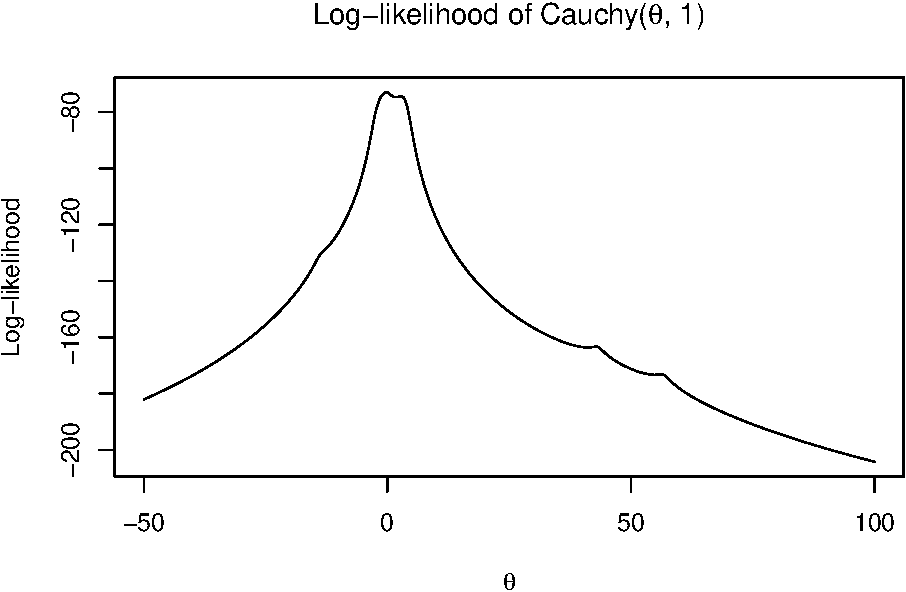
\includegraphics{Atlas-PS_2_files/figure-latex/unnamed-chunk-6-1.pdf}

We note that the log-likelihood values can be negative, as they are not
likelihoods, but rather the natural logarithms of those likelihoods.

Next, we find the MLE for \(\theta\) using Newton's Method for the set
of starting values given above. We calculate the first two derivatives
of the log-likelihood function.

\begin{align*}
l^{\prime} &= - \Sigma_{x \in X} 2 \frac{x - \theta}{1 + (x - \theta) ^2} \\
l^{\prime \prime} &= 
  - \Sigma_{x \in X} 2(1 + (x - \theta)^2)^{-1} + 
    -4 (x - \theta)(1 + (x - \theta)^2)^{-2}(x - \theta) \\
    &= - \Sigma_{x \in X} \frac{2}{1 + (x - \theta)^2} - 
    \frac{4(x - \theta)^2}{(1 + (x - \theta)^2)^2}
\end{align*}

\begin{Shaded}
\begin{Highlighting}[]
\NormalTok{newtons <-}\StringTok{ }\ControlFlowTok{function}\NormalTok{(xt, fprime, f2prime, }\DataTypeTok{tol=}\FloatTok{0.01}\NormalTok{)\{}
  \CommentTok{# Define the updating equation}
\NormalTok{  n <-}\StringTok{ }\DecValTok{0}
\NormalTok{  xt_update <-}\StringTok{ }\NormalTok{xt }\OperatorTok{+}\StringTok{ }\DecValTok{100}  
  
  \CommentTok{# While not below the tolerance level, continue updates}
  \ControlFlowTok{while}\NormalTok{(}\KeywordTok{abs}\NormalTok{(}\KeywordTok{fprime}\NormalTok{(xt)) }\OperatorTok{>}\StringTok{ }\NormalTok{tol)\{}
\NormalTok{    xt <-}\StringTok{ }\KeywordTok{ifelse}\NormalTok{(n }\OperatorTok{==}\StringTok{ }\DecValTok{0}\NormalTok{, xt, xt_update)}
    
    \CommentTok{# Define the updating equation}
\NormalTok{    xt_update <-}\StringTok{ }\NormalTok{xt }\OperatorTok{-}\StringTok{ }\NormalTok{(}\KeywordTok{fprime}\NormalTok{(xt) }\OperatorTok{/}\StringTok{ }\KeywordTok{f2prime}\NormalTok{(xt))}
\NormalTok{    n <-}\StringTok{ }\NormalTok{n }\OperatorTok{+}\StringTok{ }\DecValTok{1}
\NormalTok{  \}}
  \CommentTok{# If the adjustment value is less than the tolerance, end the iterations}
  \KeywordTok{print}\NormalTok{(}\KeywordTok{paste0}\NormalTok{(}\StringTok{"The solution is "}\NormalTok{, }\KeywordTok{round}\NormalTok{(xt_update, }\DecValTok{3}\NormalTok{) , }\StringTok{" and it was found in "}\NormalTok{, n, }\StringTok{" iterations."}\NormalTok{))}
  \KeywordTok{return}\NormalTok{(xt_update)}
\NormalTok{\}}

\CommentTok{# Define the first derivative}
\NormalTok{fprime <-}\StringTok{ }\ControlFlowTok{function}\NormalTok{(theta) }\KeywordTok{sum}\NormalTok{(}\DecValTok{2} \OperatorTok{*}\StringTok{ }\NormalTok{(X }\OperatorTok{-}\StringTok{ }\NormalTok{theta) }\OperatorTok{/}\StringTok{ }\NormalTok{(}\DecValTok{1} \OperatorTok{+}\StringTok{ }\NormalTok{(X }\OperatorTok{-}\StringTok{ }\NormalTok{theta) }\OperatorTok{^}\StringTok{ }\DecValTok{2}\NormalTok{))}

\CommentTok{# Define the second derivative}
\NormalTok{f2prime <-}\StringTok{ }\ControlFlowTok{function}\NormalTok{(theta)\{}
  \KeywordTok{return}\NormalTok{(}\DecValTok{2} \OperatorTok{*}\StringTok{ }\KeywordTok{sum}\NormalTok{ (((X }\OperatorTok{-}\StringTok{ }\NormalTok{theta) }\OperatorTok{^}\StringTok{ }\DecValTok{2} \OperatorTok{-}\StringTok{ }\DecValTok{1}\NormalTok{) }\OperatorTok{/}\StringTok{ }\NormalTok{(}\DecValTok{1} \OperatorTok{+}\StringTok{ }\NormalTok{(X }\OperatorTok{-}\StringTok{ }\NormalTok{theta) }\OperatorTok{^}\StringTok{ }\DecValTok{2}\NormalTok{ ) }\OperatorTok{^}\StringTok{ }\DecValTok{2}\NormalTok{))}
\NormalTok{\}}

\CommentTok{# Define the strating point, including mean and median}
\NormalTok{starting_points <-}\StringTok{ }\KeywordTok{c}\NormalTok{(}\OperatorTok{-}\DecValTok{11}\NormalTok{, }\OperatorTok{-}\DecValTok{1}\NormalTok{, }\DecValTok{0}\NormalTok{, }\FloatTok{1.5}\NormalTok{, }\DecValTok{4}\NormalTok{, }\FloatTok{4.7}\NormalTok{, }\DecValTok{7}\NormalTok{, }\DecValTok{8}\NormalTok{, }\DecValTok{38}\NormalTok{, }\KeywordTok{mean}\NormalTok{(X), }\KeywordTok{median}\NormalTok{(X))}

\CommentTok{# Call over all the starting points}
\NormalTok{solutions <-}\StringTok{ }\KeywordTok{sapply}\NormalTok{(starting_points, }\ControlFlowTok{function}\NormalTok{(x0)\{}
  \KeywordTok{print}\NormalTok{(}\KeywordTok{paste0}\NormalTok{(}\StringTok{"Starting Point: "}\NormalTok{, x0))}
  \KeywordTok{newtons}\NormalTok{(x0, }\DataTypeTok{fprime=}\NormalTok{fprime, }\DataTypeTok{f2prime=}\NormalTok{f2prime, }\DataTypeTok{tol=}\NormalTok{.}\DecValTok{0001}\NormalTok{)}
\NormalTok{\})}
\end{Highlighting}
\end{Shaded}

\begin{verbatim}
## [1] "Starting Point: -11"
## [1] "The solution is -821178.891 and it was found in 17 iterations."
## [1] "Starting Point: -1"
## [1] "The solution is -0.192 and it was found in 4 iterations."
## [1] "Starting Point: 0"
## [1] "The solution is -0.192 and it was found in 3 iterations."
## [1] "Starting Point: 1.5"
## [1] "The solution is 1.714 and it was found in 4 iterations."
## [1] "Starting Point: 4"
## [1] "The solution is 2.817 and it was found in 5 iterations."
## [1] "Starting Point: 4.7"
## [1] "The solution is -0.192 and it was found in 5 iterations."
## [1] "Starting Point: 7"
## [1] "The solution is 41.041 and it was found in 8 iterations."
## [1] "Starting Point: 8"
## [1] "The solution is -1145180.117 and it was found in 18 iterations."
## [1] "Starting Point: 38"
## [1] "The solution is 42.795 and it was found in 5 iterations."
## [1] "Starting Point: 5.106"
## [1] "The solution is 54.877 and it was found in 8 iterations."
## [1] "Starting Point: 1.02"
## [1] "The solution is 1.714 and it was found in 5 iterations."
\end{verbatim}

\begin{Shaded}
\begin{Highlighting}[]
\CommentTok{# Plot the likelihood function}
\NormalTok{theta_space <-}\StringTok{ }\KeywordTok{seq}\NormalTok{(}\OperatorTok{-}\DecValTok{50}\NormalTok{, }\DecValTok{50}\NormalTok{, .}\DecValTok{25}\NormalTok{)}
\NormalTok{theta_f <-}\StringTok{ }\KeywordTok{sapply}\NormalTok{(theta_space, }\ControlFlowTok{function}\NormalTok{(theta)\{}\KeywordTok{log_likelihood}\NormalTok{(theta, X)\})}
\KeywordTok{plot}\NormalTok{(theta_space, theta_f, }\StringTok{'l'}\NormalTok{, }
    \DataTypeTok{main=}\KeywordTok{TeX}\NormalTok{(}\StringTok{'Log-likelihood of Cauchy($}\CharTok{\textbackslash{}\textbackslash{}}\StringTok{theta$, 1)'}\NormalTok{ ), }
    \DataTypeTok{xlab=}\KeywordTok{TeX}\NormalTok{(}\StringTok{'$}\CharTok{\textbackslash{}\textbackslash{}}\StringTok{theta$'}\NormalTok{), }\DataTypeTok{ylab=}\StringTok{'Log-likelihood'}\NormalTok{)}

\CommentTok{# Add in all solutions found}
\KeywordTok{abline}\NormalTok{(}\DataTypeTok{v=}\NormalTok{solutions, }\DataTypeTok{col=}\StringTok{'red'}\NormalTok{, }\DataTypeTok{lty=}\DecValTok{2}\NormalTok{, }\DataTypeTok{lwd=}\NormalTok{.}\DecValTok{5}\NormalTok{)}
\end{Highlighting}
\end{Shaded}

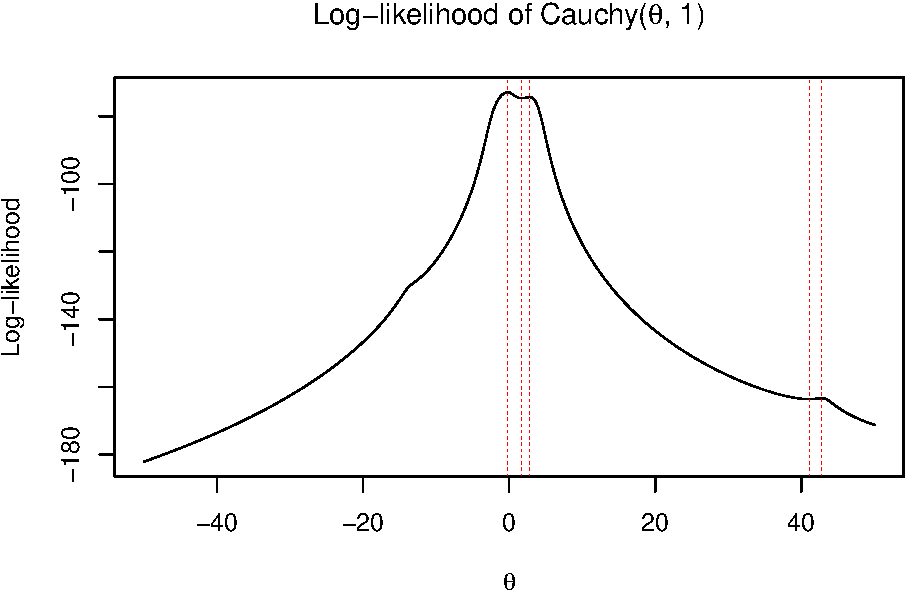
\includegraphics{Atlas-PS_2_files/figure-latex/unnamed-chunk-7-1.pdf}

We get some strange results. Depending on where the search begins, the
results are pretty wildly different. starting at 0, 1 and 4.7 yield the
correct answer. Of the other ones, some find local maxima, and some just
veer off to where the density is so low, that the derivative is
basically zero and therefore below the tolerance.

We also try the mean and the median of the data sample as starting
points. Neither of them find the actual global maximum. For a Cauchy
dsitribution, the MLE for \(\theta\) is actually the median, so the mean
is somewhat lacking as an estimator here (in fact, the expected value of
the distribution is undefined). Here, the median as a starting point
actually outperforms the mean.

Here, we plot the first derivative, which gives some insight into the
difficulty of solving this by Newton's method, which really just finds
the roots of the first derivative.

\begin{Shaded}
\begin{Highlighting}[]
\KeywordTok{plot}\NormalTok{(theta_space, }\KeywordTok{sapply}\NormalTok{(theta_space, fprime), }\StringTok{'l'}\NormalTok{, }
     \DataTypeTok{main=}\KeywordTok{TeX}\NormalTok{(}\StringTok{'$l^\{}\CharTok{\textbackslash{}\textbackslash{}}\StringTok{prime\}(}\CharTok{\textbackslash{}\textbackslash{}}\StringTok{theta)$'}\NormalTok{), }
     \DataTypeTok{xlab=}\KeywordTok{TeX}\NormalTok{(}\StringTok{'$}\CharTok{\textbackslash{}\textbackslash{}}\StringTok{theta$'}\NormalTok{), }\DataTypeTok{ylab=}\KeywordTok{TeX}\NormalTok{(}\StringTok{"$l^\{}\CharTok{\textbackslash{}\textbackslash{}}\StringTok{prime\}(}\CharTok{\textbackslash{}\textbackslash{}}\StringTok{theta)$"}\NormalTok{)}
\NormalTok{     )}
\end{Highlighting}
\end{Shaded}

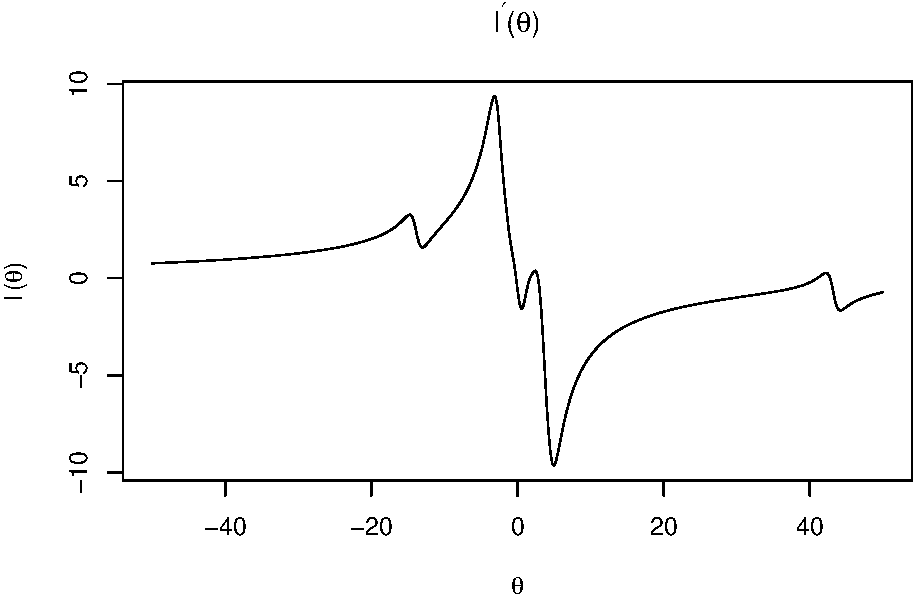
\includegraphics{Atlas-PS_2_files/figure-latex/unnamed-chunk-8-1.pdf}

The log-liklihood function does not have a well behaving first and
second derivative, and so Newton's method results in unstable solutions.
With a likelihood function like this one, it's a good idea to run many
processes over different starting points to find the correct solution.

\subsection{b)}\label{b-2}

Next, we try the bisection method. We might expect this to work better,
as we can bound the search to the part of the plot that we know contains
the maximum.

\begin{Shaded}
\begin{Highlighting}[]
\NormalTok{bisection <-}\StringTok{ }\ControlFlowTok{function}\NormalTok{(a, b, f_prime, }\DataTypeTok{tol=}\NormalTok{.}\DecValTok{0001}\NormalTok{, }\DataTypeTok{n=}\DecValTok{0}\NormalTok{)\{}
  \CommentTok{# Define the new split point}
\NormalTok{  x_t <-}\StringTok{ }\NormalTok{.}\DecValTok{5} \OperatorTok{*}\StringTok{ }\NormalTok{(a }\OperatorTok{+}\StringTok{ }\NormalTok{b)}
  \CommentTok{# Use conditioning to get the next interval}
  \ControlFlowTok{if}\NormalTok{(}\KeywordTok{f_prime}\NormalTok{(a) }\OperatorTok{*}\StringTok{ }\KeywordTok{f_prime}\NormalTok{(x_t) }\OperatorTok{<=}\StringTok{ }\DecValTok{0}\NormalTok{)\{}
\NormalTok{    new_interval <-}\StringTok{ }\KeywordTok{c}\NormalTok{(a, x_t)}
\NormalTok{  \}}\ControlFlowTok{else}\NormalTok{\{}
\NormalTok{    new_interval <-}\StringTok{ }\KeywordTok{c}\NormalTok{(x_t, b)}
\NormalTok{  \}}
  
  \CommentTok{# if interval is less than the tolerance, stop the recursion.}
  \ControlFlowTok{if}\NormalTok{ ((b }\OperatorTok{-}\StringTok{ }\NormalTok{a) }\OperatorTok{<}\StringTok{ }\NormalTok{tol)\{}
    \KeywordTok{print}\NormalTok{(}\KeywordTok{paste0}\NormalTok{(}\StringTok{"The solution is "}\NormalTok{, }\KeywordTok{round}\NormalTok{(x_t, }\DecValTok{3}\NormalTok{) , }\StringTok{" and it was found in "}\NormalTok{, n, }\StringTok{" iterations."}\NormalTok{))}
    \KeywordTok{return}\NormalTok{(x_t)}
\NormalTok{  \}}\ControlFlowTok{else}\NormalTok{\{}
    \CommentTok{# If not, call again on the new interval}
    \KeywordTok{return}\NormalTok{(}\KeywordTok{bisection}\NormalTok{(new_interval[}\DecValTok{1}\NormalTok{], new_interval[}\DecValTok{2}\NormalTok{], f_prime, }\DataTypeTok{n=}\NormalTok{n }\OperatorTok{+}\StringTok{ }\DecValTok{1}\NormalTok{))  }
\NormalTok{  \}}
\NormalTok{\}}

\CommentTok{# Define the observed values}
\NormalTok{X <-}\StringTok{ }\KeywordTok{c}\NormalTok{(}\FloatTok{1.77}\NormalTok{, }\OperatorTok{-}\NormalTok{.}\DecValTok{23}\NormalTok{, }\FloatTok{2.76}\NormalTok{, }\FloatTok{3.80}\NormalTok{, }\FloatTok{3.47}\NormalTok{, }\FloatTok{56.75}\NormalTok{, }\OperatorTok{-}\FloatTok{1.34}\NormalTok{, }\FloatTok{4.24}\NormalTok{, }
        \OperatorTok{-}\FloatTok{2.44}\NormalTok{, }\FloatTok{3.29}\NormalTok{, }\FloatTok{3.71}\NormalTok{, }\OperatorTok{-}\FloatTok{2.40}\NormalTok{, }\FloatTok{4.53}\NormalTok{, }\OperatorTok{-}\NormalTok{.}\DecValTok{07}\NormalTok{, }\OperatorTok{-}\FloatTok{1.05}\NormalTok{, }
        \OperatorTok{-}\FloatTok{13.87}\NormalTok{, }\OperatorTok{-}\FloatTok{2.53}\NormalTok{, }\OperatorTok{-}\FloatTok{1.75}\NormalTok{, .}\DecValTok{27}\NormalTok{, }\FloatTok{43.21}\NormalTok{)}

\CommentTok{# Define the derivative of the function}
\NormalTok{fprime <-}\StringTok{ }\ControlFlowTok{function}\NormalTok{(theta) }\KeywordTok{sum}\NormalTok{(}\DecValTok{2} \OperatorTok{*}\StringTok{ }\NormalTok{(X }\OperatorTok{-}\StringTok{ }\NormalTok{theta) }\OperatorTok{/}\StringTok{ }\NormalTok{(}\DecValTok{1} \OperatorTok{+}\StringTok{ }\NormalTok{(X }\OperatorTok{-}\StringTok{ }\NormalTok{theta) }\OperatorTok{^}\StringTok{ }\DecValTok{2}\NormalTok{))}

\CommentTok{# Create the likelihood function over the space}
\NormalTok{theta_space <-}\StringTok{ }\KeywordTok{seq}\NormalTok{(}\OperatorTok{-}\DecValTok{2}\NormalTok{, }\DecValTok{2}\NormalTok{, .}\DecValTok{01}\NormalTok{)}
\NormalTok{theta_f <-}\StringTok{ }\KeywordTok{sapply}\NormalTok{(theta_space, }\ControlFlowTok{function}\NormalTok{(theta)\{}\KeywordTok{log_likelihood}\NormalTok{(theta, X)\})}

\CommentTok{# Assign starting interval}
\NormalTok{a <-}\StringTok{ }\OperatorTok{-}\DecValTok{1}\NormalTok{; b <-}\StringTok{ }\DecValTok{1}\NormalTok{;}

\CommentTok{# Solve over that interval}
\NormalTok{solutions <-}\StringTok{ }\KeywordTok{bisection}\NormalTok{(a, b, }\ControlFlowTok{function}\NormalTok{(theta) }\KeywordTok{fprime}\NormalTok{(theta), }\DataTypeTok{tol=}\NormalTok{.}\DecValTok{00001}\NormalTok{)}
\end{Highlighting}
\end{Shaded}

\begin{verbatim}
## [1] "The solution is -0.192 and it was found in 15 iterations."
\end{verbatim}

\begin{Shaded}
\begin{Highlighting}[]
\CommentTok{# Plot the likelihood function}
\KeywordTok{plot}\NormalTok{(theta_space, theta_f, }\StringTok{'l'}\NormalTok{, }
    \DataTypeTok{main=}\KeywordTok{TeX}\NormalTok{(}\StringTok{'Log-likelihood of Cauchy($}\CharTok{\textbackslash{}\textbackslash{}}\StringTok{theta$, 1)'}\NormalTok{ ), }
    \DataTypeTok{xlab=}\KeywordTok{TeX}\NormalTok{(}\StringTok{'$}\CharTok{\textbackslash{}\textbackslash{}}\StringTok{theta$'}\NormalTok{), }\DataTypeTok{ylab=}\StringTok{'Log-likelihood'}\NormalTok{)}

\CommentTok{# ADd the interval lines in black}
\KeywordTok{abline}\NormalTok{(}\DataTypeTok{v=}\KeywordTok{c}\NormalTok{(a, b), }\DataTypeTok{col=}\StringTok{'red'}\NormalTok{)}
\CommentTok{# Add the solution lines in red}
\KeywordTok{abline}\NormalTok{(}\DataTypeTok{v=}\NormalTok{solutions, }\DataTypeTok{col=}\StringTok{'red'}\NormalTok{, }\DataTypeTok{lty=}\DecValTok{2}\NormalTok{)}
\end{Highlighting}
\end{Shaded}

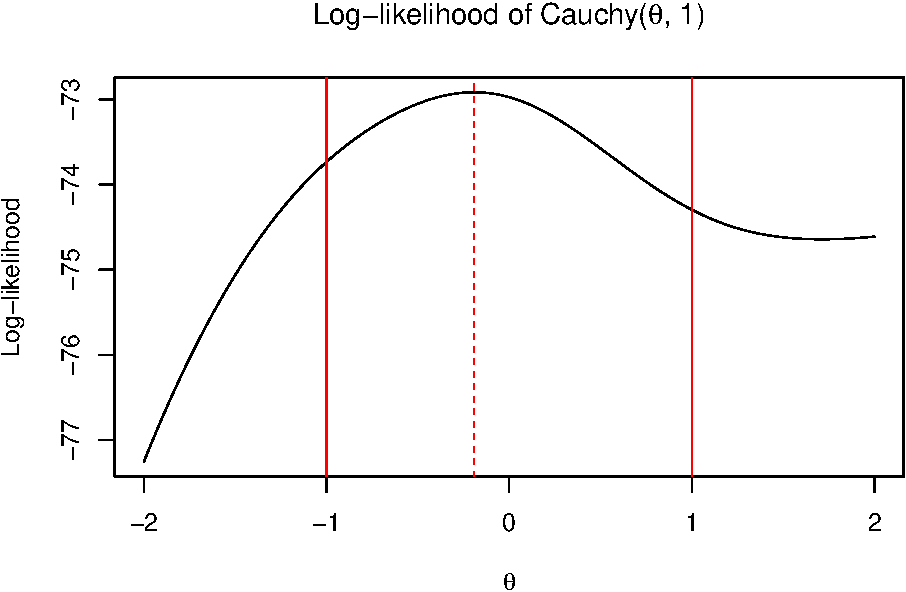
\includegraphics{Atlas-PS_2_files/figure-latex/plot_bisection-1.pdf}

Using the bisection method yields much better results, as we converge on
-.19. By visual inspection, this appears to be correct. It is worth
noting that it takes many more iterations to converge than for the
iterations of Newton's method that converged on the correct answer.

Next, we try several other intervals for the search, trying to trip up
the algorithm.

\begin{Shaded}
\begin{Highlighting}[]
\NormalTok{fprime <-}\StringTok{ }\ControlFlowTok{function}\NormalTok{(theta) }\KeywordTok{sum}\NormalTok{(}\DecValTok{2} \OperatorTok{*}\StringTok{ }\NormalTok{(X }\OperatorTok{-}\StringTok{ }\NormalTok{theta) }\OperatorTok{/}\StringTok{ }\NormalTok{(}\DecValTok{1} \OperatorTok{+}\StringTok{ }\NormalTok{(X }\OperatorTok{-}\StringTok{ }\NormalTok{theta) }\OperatorTok{^}\StringTok{ }\DecValTok{2}\NormalTok{))}
\NormalTok{theta_space <-}\StringTok{ }\KeywordTok{seq}\NormalTok{(}\OperatorTok{-}\DecValTok{100}\NormalTok{, }\DecValTok{100}\NormalTok{, .}\DecValTok{1}\NormalTok{)}
\NormalTok{theta_f <-}\StringTok{ }\KeywordTok{sapply}\NormalTok{(theta_space, }\ControlFlowTok{function}\NormalTok{(theta)\{}\KeywordTok{log_likelihood}\NormalTok{(theta, X)\})}
\KeywordTok{plot}\NormalTok{(theta_space, theta_f, }\StringTok{'l'}\NormalTok{, }
\DataTypeTok{main=}\KeywordTok{TeX}\NormalTok{(}\StringTok{'Log-likelihood of Cauchy($}\CharTok{\textbackslash{}\textbackslash{}}\StringTok{theta$, 1)'}\NormalTok{), }
\DataTypeTok{xlab=}\KeywordTok{TeX}\NormalTok{(}\StringTok{'$}\CharTok{\textbackslash{}\textbackslash{}}\StringTok{theta$'}\NormalTok{), }\DataTypeTok{ylab=}\StringTok{'Log-likelihood'}\NormalTok{)}

\CommentTok{# Iterate over the list of intervals}
\NormalTok{holder <-}\StringTok{ }\KeywordTok{lapply}\NormalTok{(}\KeywordTok{list}\NormalTok{(}
        \DataTypeTok{interval2 =} \KeywordTok{c}\NormalTok{(}\OperatorTok{-}\DecValTok{10}\NormalTok{, }\DecValTok{10}\NormalTok{, }\StringTok{'green'}\NormalTok{),}
        \DataTypeTok{interval3 =} \KeywordTok{c}\NormalTok{(}\OperatorTok{-}\DecValTok{100}\NormalTok{, }\DecValTok{100}\NormalTok{, }\StringTok{'blue'}\NormalTok{), }
        \DataTypeTok{interval4 =} \KeywordTok{c}\NormalTok{(}\DecValTok{20}\NormalTok{, }\DecValTok{80}\NormalTok{, }\StringTok{'gray'}\NormalTok{)}
\NormalTok{     ), }
     \CommentTok{# Create a function to plot the results of the intervals}
     \ControlFlowTok{function}\NormalTok{(interval)\{}
       \CommentTok{# Define the interval}
\NormalTok{       a <-}\StringTok{ }\KeywordTok{as.numeric}\NormalTok{(interval[}\DecValTok{1}\NormalTok{]); b <-}\StringTok{ }\KeywordTok{as.numeric}\NormalTok{(interval[}\DecValTok{2}\NormalTok{]);}
       \CommentTok{# Solve the problem }
\NormalTok{       solutions <-}\StringTok{ }\KeywordTok{bisection}\NormalTok{(a, b, }\ControlFlowTok{function}\NormalTok{(theta) }\KeywordTok{fprime}\NormalTok{(theta), }\DataTypeTok{tol=}\NormalTok{.}\DecValTok{00001}\NormalTok{)}
       
       \CommentTok{# Add thin solid lines for interval bounds}
       \KeywordTok{abline}\NormalTok{(}\DataTypeTok{v=}\KeywordTok{c}\NormalTok{(a, b), }\DataTypeTok{col=}\NormalTok{interval[}\DecValTok{3}\NormalTok{])}
       \CommentTok{# Add thick dashed lines for solution}
       \KeywordTok{abline}\NormalTok{(}\DataTypeTok{v=}\NormalTok{solutions, }\DataTypeTok{col=}\NormalTok{interval[}\DecValTok{3}\NormalTok{], }\DataTypeTok{lty=}\DecValTok{2}\NormalTok{, }\DataTypeTok{lwd=}\DecValTok{2}\NormalTok{)\})}
\end{Highlighting}
\end{Shaded}

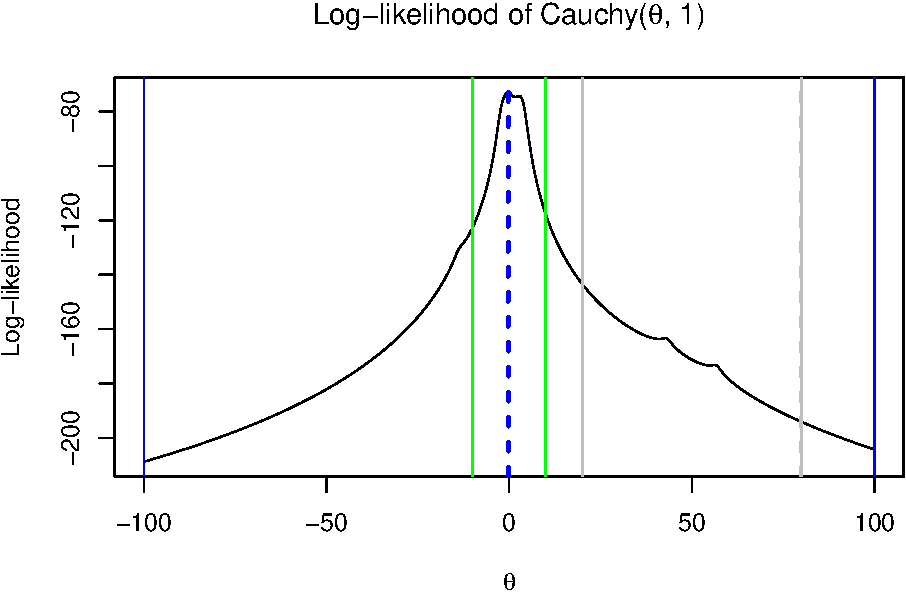
\includegraphics{Atlas-PS_2_files/figure-latex/plot_bisection_intervals-1.pdf}

\begin{verbatim}
## [1] "The solution is -0.192 and it was found in 18 iterations."
## [1] "The solution is -0.192 and it was found in 21 iterations."
## [1] "The solution is 80 and it was found in 20 iterations."
\end{verbatim}

Here, we plot the interval bounds as solid lines, and the solution as
dashed lines. Each color represents a different interval. The intervals
that include the solution solve the problem correctly. The interval that
doesn't converges on one of the endpoints.

\subsection{c)}\label{c-1}

We implement the fixed point iteration solver from starting point
\(x_0 = -1\), with scaling values \(\alpha \in \{1, .64, .25\}\).

\begin{Shaded}
\begin{Highlighting}[]
\NormalTok{fixed_point_iteration <-}\StringTok{ }\ControlFlowTok{function}\NormalTok{(x0, fprime, }\DataTypeTok{alpha=}\DecValTok{1}\NormalTok{, }\DataTypeTok{max_iter=}\DecValTok{100000}\NormalTok{, }\DataTypeTok{tol=}\NormalTok{.}\DecValTok{001}\NormalTok{)\{}
\NormalTok{  starting_point <-}\StringTok{ }\NormalTok{x0}
\NormalTok{  n <-}\StringTok{ }\DecValTok{0}
\NormalTok{  xt <-}\StringTok{ }\NormalTok{x0}
  \ControlFlowTok{while}\NormalTok{((n }\OperatorTok{<}\StringTok{ }\DecValTok{1} \OperatorTok{|}\StringTok{ }\KeywordTok{abs}\NormalTok{(x0 }\OperatorTok{-}\StringTok{ }\NormalTok{xt) }\OperatorTok{>}\StringTok{ }\NormalTok{tol) }\OperatorTok{&}\StringTok{ }\NormalTok{n }\OperatorTok{<}\StringTok{ }\NormalTok{max_iter)\{}
    \CommentTok{# Update the point}
\NormalTok{    x0 <-}\StringTok{ }\NormalTok{xt}
    
    \CommentTok{# Define update equation}
\NormalTok{    xt <-}\StringTok{ }\NormalTok{x0 }\OperatorTok{+}\StringTok{ }\NormalTok{(alpha }\OperatorTok{*}\StringTok{ }\KeywordTok{fprime}\NormalTok{(x0))}
    
\NormalTok{    n <-}\StringTok{ }\NormalTok{n }\OperatorTok{+}\StringTok{ }\DecValTok{1}
\NormalTok{  \}}
  \KeywordTok{return}\NormalTok{(}\KeywordTok{c}\NormalTok{(}\DataTypeTok{xt=}\NormalTok{xt,  }\DataTypeTok{n=}\NormalTok{n, }\DataTypeTok{starting_point=}\NormalTok{starting_point, }\DataTypeTok{alpha=}\NormalTok{alpha))}
\NormalTok{\}}

\CommentTok{# Define the derivative of the function to optimize. }

\NormalTok{fprime <-}\StringTok{ }\ControlFlowTok{function}\NormalTok{(theta) }\KeywordTok{sum}\NormalTok{(}\DecValTok{2} \OperatorTok{*}\StringTok{ }\NormalTok{(X }\OperatorTok{-}\StringTok{ }\NormalTok{theta) }\OperatorTok{/}\StringTok{ }\NormalTok{(}\DecValTok{1} \OperatorTok{+}\StringTok{ }\NormalTok{(X }\OperatorTok{-}\StringTok{ }\NormalTok{theta) }\OperatorTok{^}\StringTok{ }\DecValTok{2}\NormalTok{))}

\CommentTok{# start with x0 = -1.}
\NormalTok{results <-}\StringTok{ }\KeywordTok{t}\NormalTok{(}\KeywordTok{sapply}\NormalTok{(}\KeywordTok{c}\NormalTok{(}\DecValTok{1}\NormalTok{, .}\DecValTok{64}\NormalTok{, .}\DecValTok{25}\NormalTok{), }\ControlFlowTok{function}\NormalTok{(alpha)\{}
  \KeywordTok{fixed_point_iteration}\NormalTok{(}\OperatorTok{-}\DecValTok{1}\NormalTok{, }\DataTypeTok{fprime=}\NormalTok{fprime, }\DataTypeTok{alpha=}\NormalTok{alpha)  }
\NormalTok{\}))}
\end{Highlighting}
\end{Shaded}

\begin{longtable}[]{@{}rrrr@{}}
\caption{Results of Fixed Point Iteration}\tabularnewline
\toprule
Solution & Number of Iterations & Starting Point & Alpha\tabularnewline
\midrule
\endfirsthead
\toprule
Solution & Number of Iterations & Starting Point & Alpha\tabularnewline
\midrule
\endhead
-0.1926087 & 2294 & -1 & 1.00\tabularnewline
-0.1927677 & 196 & -1 & 0.64\tabularnewline
-0.1923656 & 7 & -1 & 0.25\tabularnewline
\bottomrule
\end{longtable}

All of the attempts converge on the correct solution, but the scaling
parameters greatly affect the number of iterations needed to get there.
We experiment with different starting points and scaling parameters
below.

\begin{Shaded}
\begin{Highlighting}[]
\NormalTok{results <-}\StringTok{ }\KeywordTok{t}\NormalTok{(}\KeywordTok{do.call}\NormalTok{(cbind, }\KeywordTok{lapply}\NormalTok{(}\KeywordTok{c}\NormalTok{(}\OperatorTok{-}\DecValTok{10}\NormalTok{, }\OperatorTok{-}\DecValTok{5}\NormalTok{, }\OperatorTok{-}\DecValTok{1}\NormalTok{, }\DecValTok{1}\NormalTok{, }\DecValTok{5}\NormalTok{, }\DecValTok{10}\NormalTok{), }\ControlFlowTok{function}\NormalTok{(x0)\{}
  \KeywordTok{return}\NormalTok{(}\KeywordTok{sapply}\NormalTok{(}\KeywordTok{c}\NormalTok{(.}\DecValTok{1}\NormalTok{, .}\DecValTok{3}\NormalTok{, .}\DecValTok{8}\NormalTok{, }\DecValTok{1}\NormalTok{), }\ControlFlowTok{function}\NormalTok{(alpha)\{}
    \KeywordTok{fixed_point_iteration}\NormalTok{(x0, }\DataTypeTok{fprime=}\NormalTok{fprime, }\DataTypeTok{alpha=}\NormalTok{alpha, }\DataTypeTok{max_iter=}\DecValTok{100000}\NormalTok{)  }
\NormalTok{  \}))  }
\NormalTok{\})))}
\end{Highlighting}
\end{Shaded}

\begin{longtable}[]{@{}rrrr@{}}
\caption{Results of Fixed Point Iteration}\tabularnewline
\toprule
Solution & Number of Iterations & Starting Point & Alpha\tabularnewline
\midrule
\endfirsthead
\toprule
Solution & Number of Iterations & Starting Point & Alpha\tabularnewline
\midrule
\endhead
-0.1939787 & 37 & -10 & 0.1\tabularnewline
-0.1923074 & 11 & -10 & 0.3\tabularnewline
0.3720408 & 100000 & -10 & 0.8\tabularnewline
2.6415064 & 100000 & -10 & 1.0\tabularnewline
-0.1941545 & 24 & -5 & 0.1\tabularnewline
-0.1923103 & 5 & -5 & 0.3\tabularnewline
-0.8024924 & 100000 & -5 & 0.8\tabularnewline
-0.1920627 & 7 & -5 & 1.0\tabularnewline
-0.1939695 & 18 & -1 & 0.1\tabularnewline
-0.1923041 & 5 & -1 & 0.3\tabularnewline
-0.8024924 & 100000 & -1 & 0.8\tabularnewline
-0.1926087 & 2294 & -1 & 1.0\tabularnewline
-0.1902990 & 20 & 1 & 0.1\tabularnewline
-0.1922690 & 6 & 1 & 0.3\tabularnewline
-0.8024924 & 100000 & 1 & 0.8\tabularnewline
-0.1921332 & 9344 & 1 & 1.0\tabularnewline
2.8202633 & 20 & 5 & 0.1\tabularnewline
2.8172474 & 13 & 5 & 0.3\tabularnewline
2.8170617 & 22 & 5 & 0.8\tabularnewline
2.9290552 & 100000 & 5 & 1.0\tabularnewline
2.8202693 & 29 & 10 & 0.1\tabularnewline
2.8177720 & 9 & 10 & 0.3\tabularnewline
0.3720408 & 100000 & 10 & 0.8\tabularnewline
-0.1926818 & 21769 & 10 & 1.0\tabularnewline
\bottomrule
\end{longtable}

We can see that the starting point and scaling parameters heavily
impacts the convergence of the algorithm to the correct solution.
Smaller scaling parameters tend to work better, with with those around
\(.3\) usually converging the fastest. Additionally, a scaling parameter
of \(.8\) reliably fails from all starting points. This reiterates the
need to run parallel processes across various parameters to get a sense
for the true result.

\subsection{d)}\label{d-1}

Using starting values
\((\theta^{(0)}, \theta^{(1)}) \in \{(-2, -1), (-3, 3)\}\), we apply the
secant method to estimate \(\theta\).

\begin{Shaded}
\begin{Highlighting}[]
\NormalTok{secant_method <-}\StringTok{ }\ControlFlowTok{function}\NormalTok{(x0, x1, fprime, }\DataTypeTok{max_iter=}\DecValTok{100000}\NormalTok{, }\DataTypeTok{tol=}\NormalTok{.}\DecValTok{001}\NormalTok{)\{}
\NormalTok{  n <-}\StringTok{ }\DecValTok{0}
  
  \ControlFlowTok{while}\NormalTok{((n }\OperatorTok{<}\StringTok{ }\DecValTok{1} \OperatorTok{|}\StringTok{ }\KeywordTok{abs}\NormalTok{(x0 }\OperatorTok{-}\StringTok{ }\NormalTok{x1) }\OperatorTok{>}\StringTok{ }\NormalTok{tol) }\OperatorTok{&}\StringTok{ }\NormalTok{n }\OperatorTok{<}\StringTok{ }\NormalTok{max_iter)\{}
    \CommentTok{# Define the updating equation}
\NormalTok{    xt <-}\StringTok{ }\NormalTok{x1 }\OperatorTok{-}\StringTok{ }\KeywordTok{fprime}\NormalTok{(x1) }\OperatorTok{*}\StringTok{ }\NormalTok{(x1 }\OperatorTok{-}\StringTok{ }\NormalTok{x0) }\OperatorTok{/}\StringTok{ }\NormalTok{(}\KeywordTok{fprime}\NormalTok{(x1) }\OperatorTok{-}\StringTok{ }\KeywordTok{fprime}\NormalTok{(x0))}
    
    \CommentTok{# Iterate on update}
\NormalTok{    x0 <-}\StringTok{ }\NormalTok{x1; x1 <-}\StringTok{ }\NormalTok{xt;  }
    
\NormalTok{    n <-}\StringTok{ }\NormalTok{n }\OperatorTok{+}\StringTok{ }\DecValTok{1}
\NormalTok{  \}}
  \KeywordTok{print}\NormalTok{(}\KeywordTok{paste0}\NormalTok{(}\StringTok{"The solution is: "}\NormalTok{, xt, }\StringTok{". The algorithm converged in "}\NormalTok{, n, }\StringTok{" iterations"}\NormalTok{))}
  
  \KeywordTok{return}\NormalTok{(xt)}
\NormalTok{\}}
\end{Highlighting}
\end{Shaded}

\begin{verbatim}
## [1] "Starting points of (-2, 1)"
\end{verbatim}

\begin{verbatim}
## [1] "The solution is: -0.192286493714121. The algorithm converged in 5 iterations"
\end{verbatim}

\begin{verbatim}
## [1] "Starting points of (-3, 3)"
\end{verbatim}

\begin{verbatim}
## [1] "The solution is: 2.81746622667055. The algorithm converged in 5 iterations"
\end{verbatim}

\begin{verbatim}
## [1] "Starting Points of (-2, 3)"
\end{verbatim}

\begin{verbatim}
## [1] "The solution is: 2.81747656517513. The algorithm converged in 6 iterations"
\end{verbatim}

\begin{verbatim}
## [1] "Starting Points of (-4, -4.5)"
\end{verbatim}

\begin{verbatim}
## [1] "The solution is: -1.94676563893071e+154. The algorithm converged in 738 iterations"
\end{verbatim}

We see a pretty wide variety of results, entirely dependant on the
parameterization of the starting points. The takeaway here may be that
this method requires a very careful selection of starting points, based
on the plot of the function being maximized. The first set of points
converges quickly and to the correct answer. The rest do not. The 2nd
pair of points given in the text find a different root of the
derivative. Some other points tried find the wrong root, as well as run
off to divergence before stopping when the likelihood function levels
off.

\subsection{e)}\label{e}

To compare the results takes some nuance, as different algorithms excel
in different ways.

\begin{enumerate}
\def\labelenumi{\arabic{enumi}.}
\item
  The bisection method has stability, but comes with a performance
  drawback.
\item
  Fixed point iteration is the most unstable, as various starting points
  and scaling parameters simply fail, with small changes in inputs
  leading to large changes in outputs.
\item
  Newton's Method is extremely fast when it starts in the right place
  and isn't tripped up by unusual function behavior. Again, a win in
  performance, but less so in stability.
\item
  The secant method performs well when it finds the right thing, but it
  often doesn't, and the starting points appear to really tank the
  performance. It seems difficult to pick starting points that work,
  even when examining the function manually.
\end{enumerate}

Intuitively, stability and speed should be a trade off, as an exhaustive
search will be entirely stable, and a random selection will be entirely
unstable, so this makes sense. Additional considerations should center
around the difficulty of calculating the second derivative, as this
could be a primary motivation for using the secant method, and the
function at hand. If the function is unimodel, a fast search can likely
be employed successfully. If the search space is small and the function
is difficult, a more robust, slower search may be a better option.

\section{Problem 4}\label{problem-4}

\subsection{\texorpdfstring{a) We find the MLE for \(\lambda\), given a
Poisson distribution. The PDF of a Poisson distribution
is}{a) We find the MLE for \textbackslash{}lambda, given a Poisson distribution. The PDF of a Poisson distribution is}}\label{a-we-find-the-mle-for-lambda-given-a-poisson-distribution.-the-pdf-of-a-poisson-distribution-is}

\[
f(x; \lambda) = \frac{\lambda^{x}\rm{e}^{-\lambda}}{x!}.
\] Therefore, the likelihood function \(L(\lambda)\) is the product of
the likelihods for each data sample: \[
  L(\lambda) = \prod_{i=1}^{n} \frac{\lambda^{x_i}\rm{e}^{-\lambda}}{x_i!}.
\] and the log-likelihood can be written as the sum of the logs:

\begin{align*}
l(\lambda) &=  \log{\prod_{i=1}^{n} \frac{\lambda^{x_i}\rm{e}^{-\lambda}}{x_i!}} \\
          &= \summ \log{\lambda^{x_i}} - \summ \log{X_i!} - \summ \lambda \\
          &=  \summ x_i \log{\lambda} - \summ \log{X_i!} - n \lambda.
\end{align*}

We find the first derivative of the log-likelihood function: \[
l^{\prime}(\lambda) = \summ \frac{x_i}{\lambda} - n,
\] and then find the root: \[
 0 = \summ \frac{x_i}{\lambda} - n \implies \lambda = \summ \frac{x_i}{n}.
 \] Therefore, the MLE for \(\lambda\) is \(\summ(x_i) / n\), which is
the mean of the data sample. This is as expected, as the expected value
of a Poisson distribution is \(\lambda\).

\subsection{b)}\label{b-3}

Next, we look for the MLE of \(\theta\) in an Exponential Distribution.
The PDF of an Exponential distribution is \[
f(x; \theta) = \theta \rm{e}^{-\theta x}.
\]

We can write the likelihood function for \(\theta\) as \[
L(\theta) = \prod_{i=1}^{n}\theta\rm{e}^{-\theta x_i}, 
\] with the log-likelihood as

\begin{align*}
l(\theta) &= \log{\prod_{i=1}^{n}\theta\rm{e}^{-\theta x_i}} \\
&= \summ \log{\theta} + \summ{-\theta x_i} \\
&= n \log{\theta} - \theta \summ x_i.
\end{align*}

To find the MLE, we find the root of the first derivative: \[
0 = l^{\prime}(\theta) = \frac{n}{\theta} -  \summ x_i \implies \theta = \frac{n}{\summ x_i}.
\] Solving this equation gives us the MLE for \(\theta\) as
\(\theta = \frac{n}{\summ x_i}\). This is as expected, as the expected
value of an Exponential(\(\theta\)) distribution is
\(\frac{1}{\theta}\), and so the MLE for \(\theta\) is the reciprocal of
the mean.

\section{Problem 5}\label{problem-5}

To find the Fisher Information \(I(\theta)\), we use the formula \[
I(\theta) = E[(l^{\prime}(\theta))^2].
\]

First, we find \(L(\theta)\) for a set of \(n\) independent Bernoulli
trials with parameter \(\theta\). This is simply the likelihood function
for a Binomial distribution: \[
L(\theta; x, n) = {n\choose x} \theta^x (1-\theta)^{n-x}, 
\] with log-likelihood \[
l(\theta) = \log{n \choose k} + x\log{\theta} + (n - x) \log{(1 - \theta)}.
\]

We first take the first derivative of the log-likelihood function, \[
l^{\prime}(\theta) = \frac{x}{\theta} - \frac{n - x}{1- \theta} = 
\frac{x (1 - \theta)}{\theta(1 - \theta)} - \frac{n\theta - x\theta}{\theta (1 - \theta)} = \frac{x - n \theta}{\theta(1 - \theta)}, 
\] and then square it \[
\left(\frac{x - n \theta}{\theta(1 - \theta)}\right)^2 = \frac{x^2}{\theta^2 (1 - \theta)^2} - \frac{2nx}{\theta(1-\theta)^2} - \frac{n^2}{(1-\theta)^2}.
\] We then take the expected value of this. Using the algebraic
properties of the Expected Value function, we can write \[
E((l^{\prime}(\theta)^2) = \frac{1}{\theta^2(1 - \theta)^2}E(X^2) - \frac{2n}{\theta(1-\theta)^2}E(X) + \frac{n^2}{(1 - \theta)^2}.
\]

We site the textbook's table of distribution to define the following:

\begin{align*} 
E(X) &= n \theta \\
Var(X) &= n \theta (1 - \theta).
\end{align*}

Note that \(Var(X) = E(X^2) - E(X) ^2\), and so
\(E(X^2) = Var(X) + E(X)^2 = n\theta(1 - \theta) + n^2 \theta^2\). We
can then plug these into the formulas above, such that

\begin{align*}
E((l^{\prime}(\theta)^2) &= \frac{1}{\theta^2(1 - \theta)^2}E(X^2) - \frac{2n}{\theta(1-\theta)^2}E(X) + \frac{n^2}{(1 - \theta)^2} \\
&= \frac{n\theta(1 - \theta)  + n^2 \theta^2}{\theta^2(1 - \theta)^2} - 
          \frac{2n^2\theta^2}{\theta^2(1-\theta)^2} + 
          \frac{n^2 \theta^2}{\theta^2(1-\theta)^2} \\
&= \frac{n \theta ( 1- \theta)}{\theta^2 ( 1- \theta)^2} \\
&= \frac{n}{\theta(1-\theta)}.
\end{align*}

Therefore, the Fisher Information can be described as
\(I(\theta)=\frac{n}{\theta (1 - \theta)}\).


\end{document}
